% SPDX-License-Identifier: CC-BY-4.0
%
% Copyright (c) 2023 Nelson Vieira
%
% @author Nelson Vieira <nelson0.vieira@gmail.com>
% @license CC-BY-4.0 <https://creativecommons.org/licenses/by/4.0/legalcode.txt>
\documentclass{article}
\usepackage{amsmath}
\usepackage{color,pxfonts,fix-cm}
\usepackage{latexsym}
\usepackage[mathletters]{ucs}
\DeclareUnicodeCharacter{32}{$\ $}
\DeclareUnicodeCharacter{8226}{$\bullet$}
\DeclareUnicodeCharacter{9642}{$\blacksquare$}
% \usepackage{fontspec}
\usepackage[OT1]{fontenc}
\usepackage{cmbright}
\usepackage[utf8x]{inputenc}
\usepackage{pict2e}
\usepackage{wasysym}
\usepackage[english]{babel}
\usepackage{tikz}
\pagestyle{empty}
\usepackage[margin=0in,paperwidth=960pt,paperheight=540pt]{geometry}
\def\myversion{1.0.1}

\begin{document}
\definecolor{color_283006}{rgb}{1,1,1}
\definecolor{color_214192}{rgb}{0.741177,0.345098,0.172549}
\definecolor{color_252978}{rgb}{0.894118,0.513726,0.070588}
\definecolor{color_155902}{rgb}{0.498039,0.498039,0.498039}
\definecolor{color_67525}{rgb}{0.14902,0.14902,0.14902}
\definecolor{color_128484}{rgb}{0.388235,0.439216,0.321569}
\definecolor{color_93343}{rgb}{0.25098,0.25098,0.25098}
\definecolor{color_29791}{rgb}{0,0,0}
\begin{tikzpicture}[overlay]
\path(0pt,0pt);
\filldraw[color_283006][even odd rule]
(-15pt, 10pt) -- (945pt, 10pt)
-- (945pt, 10pt)
-- (945pt, -530pt)
-- (945pt, -530pt)
-- (-15pt, -530pt) -- cycle
;
\filldraw[color_214192][even odd rule]
(-14.75pt, -494pt) -- (945pt, -494pt)
-- (945pt, -494pt)
-- (945pt, -530pt)
-- (945pt, -530pt)
-- (-14.75pt, -530pt) -- cycle
;
\filldraw[color_252978][even odd rule]
(-15pt, -488.75pt) -- (944.75pt, -488.75pt)
-- (944.75pt, -488.75pt)
-- (944.75pt, -493.75pt)
-- (944.75pt, -493.75pt)
-- (-15pt, -493.75pt) -- cycle
;
\draw[color_155902,line width=0.5pt]
(80.12503pt, -332pt) -- (857.75pt, -332pt)
;
\end{tikzpicture}
\begin{picture}(-5,0)(2.5,0)
\put(78.60001,-227.1502){\fontsize{80}{1}\selectfont\color{color_67525}Privacidade em sistemas}
\put(78.60001,-308.7502){\fontsize{80}{1}\selectfont\color{color_67525}IoT}
\put(78.82504,-365.4784){\fontsize{24}{1}\selectfont\color{color_128484}\uppercase{Mestrado em Engenharia Informática}}
\put(78.82504,-405.3984){\fontsize{24}{1}\selectfont\color{color_128484}\uppercase{Apresentação de Dissertação}}
\put(78.82504,-445.3184){\fontsize{24}{1}\selectfont\color{color_128484}\uppercase{Nelson Vieira}}
\put(71,-115.25){
\includegraphics[width=157.8749pt,height=65.25pt]{../assets/images/uma_logo.png}}
\end{picture}
\newpage
\begin{tikzpicture}[overlay]
\path(0pt,0pt);
\filldraw[color_283006][even odd rule]
(-15pt, 10pt) -- (945pt, 10pt)
-- (945pt, 10pt)
-- (945pt, -530pt)
-- (945pt, -530pt)
-- (-15pt, -530pt) -- cycle
;
\filldraw[color_214192][even odd rule]
(-15pt, -494pt) -- (945pt, -494pt)
-- (945pt, -494pt)
-- (945pt, -530pt)
-- (945pt, -530pt)
-- (-15pt, -530pt) -- cycle
;
\filldraw[color_252978][even odd rule]
(-15pt, -488.75pt) -- (945pt, -488.75pt)
-- (945pt, -488.75pt)
-- (945pt, -494pt)
-- (945pt, -494pt)
-- (-15pt, -494pt) -- cycle
;
\draw[color_155902,line width=0.5pt]
(79pt, -126.8751pt) -- (863.75pt, -126.8751pt)
;
\end{tikzpicture}
\begin{picture}(-5,0)(2.5,0)
\put(78.60001,-112.2741){\fontsize{48}{1}\selectfont\color{color_93343}Privacidade online}
\put(532,-390.75){
\includegraphics[width=386.1251pt,height=201.75pt]{assets/images/nsa_files.png}}
\put(39,-345.1251){
\includegraphics[width=304.5pt,height=100.125pt]{assets/images/wikileaks.png}}
\put(378,-395.75){
\includegraphics[width=201.75pt,height=201.75pt]{assets/images/anonymous.png}}
\end{picture}
\newpage
\begin{tikzpicture}[overlay]
\path(0pt,0pt);
\filldraw[color_283006][even odd rule]
(-15pt, 10pt) -- (945pt, 10pt)
-- (945pt, 10pt)
-- (945pt, -530pt)
-- (945pt, -530pt)
-- (-15pt, -530pt) -- cycle
;
\filldraw[color_214192][even odd rule]
(-15pt, -494pt) -- (945pt, -494pt)
-- (945pt, -494pt)
-- (945pt, -530pt)
-- (945pt, -530pt)
-- (-15pt, -530pt) -- cycle
;
\filldraw[color_252978][even odd rule]
(-15pt, -488.75pt) -- (945pt, -488.75pt)
-- (945pt, -488.75pt)
-- (945pt, -494pt)
-- (945pt, -494pt)
-- (-15pt, -494pt) -- cycle
;
\draw[color_155902,line width=0.5pt]
(79pt, -126.8751pt) -- (863.75pt, -126.8751pt)
;
\end{tikzpicture}
\begin{picture}(-5,0)(2.5,0)
\put(78.60001,-112.2741){\fontsize{48}{1}\selectfont\color{color_93343}Privacidade online}
\put(172,-361.75){
\includegraphics[width=178.375pt,height=56.75pt]{assets/images/https.png}}
\put(445,-431.25){
\includegraphics[width=334.8749pt,height=282.25pt]{assets/images/cookies_example.png}}
\put(175,-237.75){
\includegraphics[width=169.25pt,height=56.75pt]{assets/images/gdpr.png}}
\end{picture}
\newpage
\begin{tikzpicture}[overlay]
\path(0pt,0pt);
\filldraw[color_283006][even odd rule]
(-15pt, 10pt) -- (945pt, 10pt)
-- (945pt, 10pt)
-- (945pt, -530pt)
-- (945pt, -530pt)
-- (-15pt, -530pt) -- cycle
;
\filldraw[color_214192][even odd rule]
(-15pt, -494pt) -- (945pt, -494pt)
-- (945pt, -494pt)
-- (945pt, -530pt)
-- (945pt, -530pt)
-- (-15pt, -530pt) -- cycle
;
\filldraw[color_252978][even odd rule]
(-15pt, -488.75pt) -- (945pt, -488.75pt)
-- (945pt, -488.75pt)
-- (945pt, -494pt)
-- (945pt, -494pt)
-- (-15pt, -494pt) -- cycle
;
\draw[color_155902,line width=0.5pt]
(79pt, -126.8751pt) -- (863.75pt, -126.8751pt)
;
\end{tikzpicture}
\begin{picture}(-5,0)(2.5,0)
\put(78.60001,-112.2741){\fontsize{48}{1}\selectfont\color{color_93343}Internet of Things}
\put(487,-416.1249){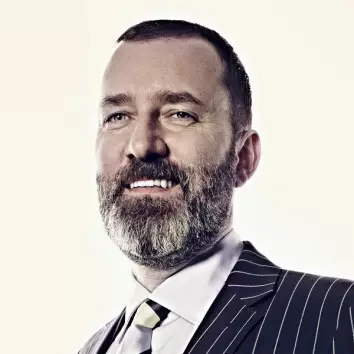
\includegraphics[width=281.25pt,height=281.1249pt]{assets/images/kevin_ashton.png}}
\put(178,-422.1251){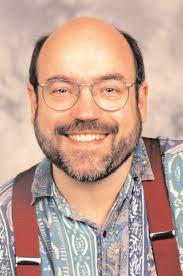
\includegraphics[width=186.375pt,height=281.1251pt]{assets/images/mark_weiser.png}}
\put(596.5751,-452.2278){\fontsize{18}{1}\selectfont\color{color_29791}Kevin Ashton}
\put(219.45,-452.2278){\fontsize{18}{1}\selectfont\color{color_29791}Mark Weiser}
\end{picture}
\newpage
\begin{tikzpicture}[overlay]
\path(0pt,0pt);
\filldraw[color_283006][even odd rule]
(-15pt, 10pt) -- (945pt, 10pt)
-- (945pt, 10pt)
-- (945pt, -530pt)
-- (945pt, -530pt)
-- (-15pt, -530pt) -- cycle
;
\filldraw[color_214192][even odd rule]
(-15pt, -494pt) -- (945pt, -494pt)
-- (945pt, -494pt)
-- (945pt, -530pt)
-- (945pt, -530pt)
-- (-15pt, -530pt) -- cycle
;
\filldraw[color_252978][even odd rule]
(-15pt, -488.75pt) -- (945pt, -488.75pt)
-- (945pt, -488.75pt)
-- (945pt, -494pt)
-- (945pt, -494pt)
-- (-15pt, -494pt) -- cycle
;
\draw[color_155902,line width=0.5pt]
(79pt, -126.8751pt) -- (863.75pt, -126.8751pt)
;
\end{tikzpicture}
\begin{picture}(-5,0)(2.5,0)
\put(78.57504,-112.2241){\fontsize{48}{1}\selectfont\color{color_93343}Porquê privacidade em sistemas IoT}
\put(588.6251,-259.1028){\fontsize{20}{1}\selectfont\color{color_93343}Sistemas de comunicação muito}
\put(588.6251,-280.7028){\fontsize{20}{1}\selectfont\color{color_93343}variados, fornecem diferentes}
\put(588.6251,-302.3028){\fontsize{20}{1}\selectfont\color{color_93343}distâncias, taxas de dados e}
\put(588.6251,-323.9028){\fontsize{20}{1}\selectfont\color{color_93343}necessidades de infraestrutura}
\put(96,-483.75){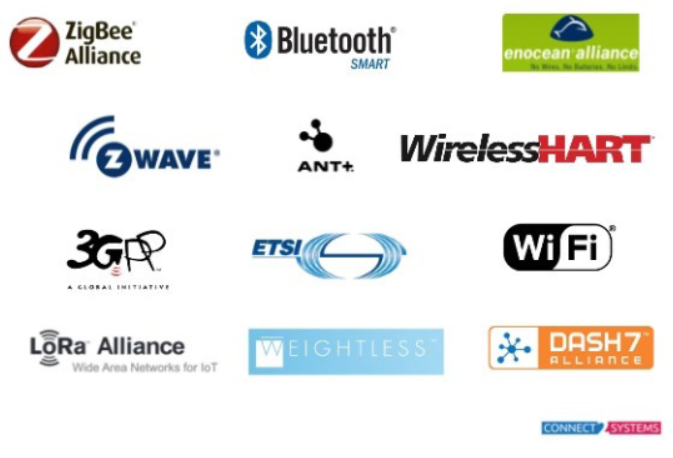
\includegraphics[width=465.5pt,height=316.75pt]{assets/images/iotnetworks.png}}
\end{picture}
\newpage
\begin{tikzpicture}[overlay]
\path(0pt,0pt);
\filldraw[color_283006][even odd rule]
(-15pt, 10pt) -- (945pt, 10pt)
-- (945pt, 10pt)
-- (945pt, -530pt)
-- (945pt, -530pt)
-- (-15pt, -530pt) -- cycle
;
\filldraw[color_214192][even odd rule]
(-15pt, -494pt) -- (945pt, -494pt)
-- (945pt, -494pt)
-- (945pt, -530pt)
-- (945pt, -530pt)
-- (-15pt, -530pt) -- cycle
;
\filldraw[color_252978][even odd rule]
(-15pt, -488.75pt) -- (945pt, -488.75pt)
-- (945pt, -488.75pt)
-- (945pt, -494pt)
-- (945pt, -494pt)
-- (-15pt, -494pt) -- cycle
;
\draw[color_155902,line width=0.5pt]
(79pt, -126.8751pt) -- (863.75pt, -126.8751pt)
;
\end{tikzpicture}
\begin{picture}(-5,0)(2.5,0)
\put(78.60001,-112.2741){\fontsize{48}{1}\selectfont\color{color_93343}O paradoxo da privacidade}
\put(98.99998,-251.8528){\fontsize{20}{1}\selectfont\color{color_93343}É a dicotomia entre as intenções de uma}
\put(98.94998,-273.4528){\fontsize{20}{1}\selectfont\color{color_93343}pessoa de proteger a sua privacidade em}
\put(98.94998,-295.0528){\fontsize{20}{1}\selectfont\color{color_93343}contraste com o comportamento desta online}
\put(98.94998,-316.6528){\fontsize{20}{1}\selectfont\color{color_93343}e, como resultado, compromete a sua}
\put(98.94998,-338.2528){\fontsize{20}{1}\selectfont\color{color_93343}privacidade}
\put(547,-463){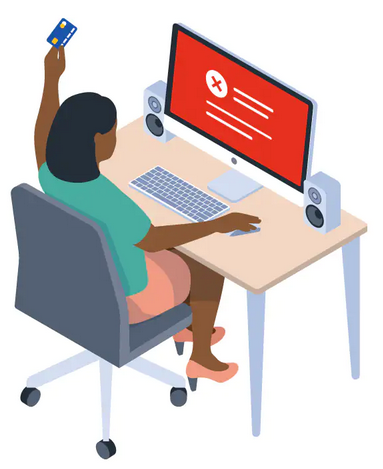
\includegraphics[width=262.125pt,height=321pt]{assets/images/privacy_paradox.png}}
\end{picture}
\newpage
\begin{tikzpicture}[overlay]
\path(0pt,0pt);
\filldraw[color_283006][even odd rule]
(-15pt, 10pt) -- (945pt, 10pt)
-- (945pt, 10pt)
-- (945pt, -530pt)
-- (945pt, -530pt)
-- (-15pt, -530pt) -- cycle
;
\filldraw[color_214192][even odd rule]
(-15pt, -494pt) -- (945pt, -494pt)
-- (945pt, -494pt)
-- (945pt, -530pt)
-- (945pt, -530pt)
-- (-15pt, -530pt) -- cycle
;
\filldraw[color_252978][even odd rule]
(-15pt, -488.75pt) -- (945pt, -488.75pt)
-- (945pt, -488.75pt)
-- (945pt, -494pt)
-- (945pt, -494pt)
-- (-15pt, -494pt) -- cycle
;
\draw[color_155902,line width=0.5pt]
(79pt, -126.8751pt) -- (863.75pt, -126.8751pt)
;
\end{tikzpicture}
\begin{picture}(-5,0)(2.5,0)
\put(78.60001,-112.2741){\fontsize{48}{1}\selectfont\color{color_93343}Metodologia}
\put(78.62503,-156.4779){\fontsize{20}{1}\selectfont\color{color_93343}\textbf{O que fazer?}}
\put(78.62503,-192.0779){\fontsize{20}{1}\selectfont\color{color_93343}Criar uma espécie de privacy assistant, mas}
\put(78.57503,-213.6779){\fontsize{20}{1}\selectfont\color{color_93343}diferente deste tipo de aplicações que existem}
\put(78.57503,-235.2778){\fontsize{20}{1}\selectfont\color{color_93343}atualmente no mercado.}
\put(78.62503,-270.8778){\fontsize{20}{1}\selectfont\color{color_93343}Tendo como principais objectivos:}
\put(71.37503,-306.4778){\fontsize{14}{1}\selectfont\color{color_252978}\unichar{8226}}
\put(78.62503,-306.4778){\fontsize{20}{1}\selectfont\color{color_93343}Detetar sistemas iot que estejam próximos do}
\put(78.57503,-328.0778){\fontsize{20}{1}\selectfont\color{color_93343}utilizador;}
\put(71.37503,-363.6778){\fontsize{14}{1}\selectfont\color{color_252978}\unichar{8226}}
\put(78.62503,-363.6778){\fontsize{20}{1}\selectfont\color{color_93343}Caracterizar estes dispositivos tendo em conta}
\put(78.57503,-385.2778){\fontsize{20}{1}\selectfont\color{color_93343}o tipo de informações que estes possam}
\put(78.57503,-406.8778){\fontsize{20}{1}\selectfont\color{color_93343}recolher;}
\put(71.37503,-442.4778){\fontsize{14}{1}\selectfont\color{color_252978}\unichar{8226}}
\put(78.62503,-442.4778){\fontsize{20}{1}\selectfont\color{color_93343}Permitir que o utilizador possa recusar a }
\put(78.57503,-464.0778){\fontsize{20}{1}\selectfont\color{color_93343}recolha dos seus dados, caso seja possível.}
\put(467,-429.6251){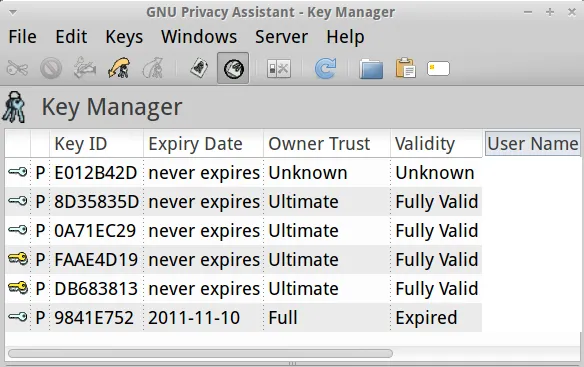
\includegraphics[width=416.25pt,height=261.6251pt]{assets/images/privacy_assistant_example.png}}
\end{picture}
\newpage
\begin{tikzpicture}[overlay]
\path(0pt,0pt);
\filldraw[color_283006][even odd rule]
(-15pt, 10pt) -- (945pt, 10pt)
-- (945pt, 10pt)
-- (945pt, -530pt)
-- (945pt, -530pt)
-- (-15pt, -530pt) -- cycle
;
\filldraw[color_214192][even odd rule]
(-15pt, -494pt) -- (945pt, -494pt)
-- (945pt, -494pt)
-- (945pt, -530pt)
-- (945pt, -530pt)
-- (-15pt, -530pt) -- cycle
;
\filldraw[color_252978][even odd rule]
(-15pt, -488.75pt) -- (945pt, -488.75pt)
-- (945pt, -488.75pt)
-- (945pt, -494pt)
-- (945pt, -494pt)
-- (-15pt, -494pt) -- cycle
;
\draw[color_155902,line width=0.5pt]
(79pt, -126.8751pt) -- (863.75pt, -126.8751pt)
;
\end{tikzpicture}
\begin{picture}(-5,0)(2.5,0)
\put(78.60001,-112.2741){\fontsize{48}{1}\selectfont\color{color_93343}Trabalhos semelhantes}
\put(78.65007,-156.4362){\fontsize{20}{1}\selectfont\color{color_93343}\textbf{LTEye}}
\put(71.40007,-263.2362){\fontsize{20}{1}\selectfont\color{color_93343}Serve para análises temporais e}
\put(71.40007,-284.8362){\fontsize{20}{1}\selectfont\color{color_93343}espaciais refinadas no desempenho de}
\put(71.40007,-306.4362){\fontsize{20}{1}\selectfont\color{color_93343}rádio LTE}
\put(388,-449.75){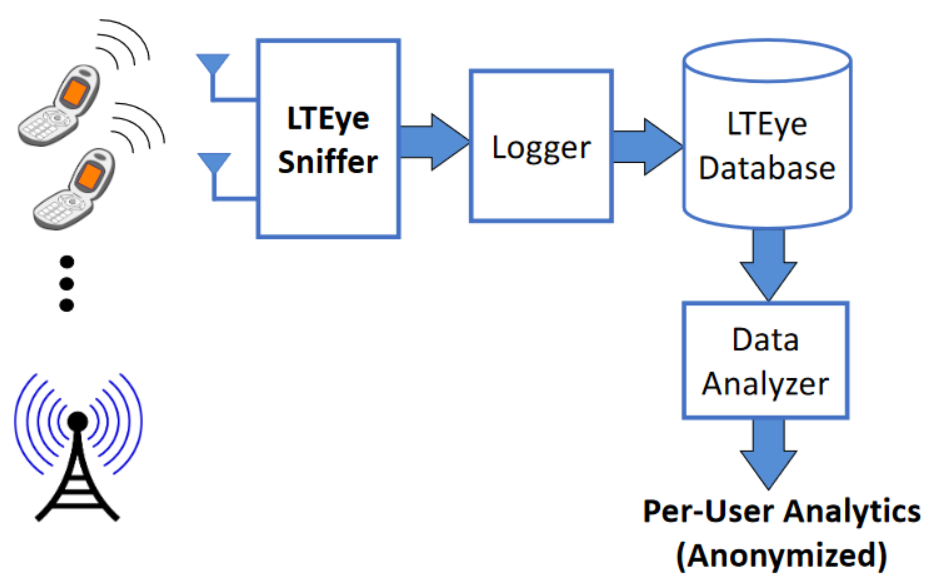
\includegraphics[width=503.5pt,height=316.75pt]{assets/images/lteye.png}}
\end{picture}
\newpage
\begin{tikzpicture}[overlay]
\path(0pt,0pt);
\filldraw[color_283006][even odd rule]
(-15pt, 10pt) -- (945pt, 10pt)
-- (945pt, 10pt)
-- (945pt, -530pt)
-- (945pt, -530pt)
-- (-15pt, -530pt) -- cycle
;
\filldraw[color_214192][even odd rule]
(-15pt, -494pt) -- (945pt, -494pt)
-- (945pt, -494pt)
-- (945pt, -530pt)
-- (945pt, -530pt)
-- (-15pt, -530pt) -- cycle
;
\filldraw[color_252978][even odd rule]
(-15pt, -488.75pt) -- (945pt, -488.75pt)
-- (945pt, -488.75pt)
-- (945pt, -494pt)
-- (945pt, -494pt)
-- (-15pt, -494pt) -- cycle
;
\draw[color_155902,line width=0.5pt]
(79pt, -126.8751pt) -- (863.75pt, -126.8751pt)
;
\end{tikzpicture}
\begin{picture}(-5,0)(2.5,0)
\put(78.60001,-112.2741){\fontsize{48}{1}\selectfont\color{color_93343}Trabalhos semelhantes}
\put(78.65007,-156.4362){\fontsize{20}{1}\selectfont\color{color_93343}\textbf{IoT Assistant}}
\put(105,-465.5){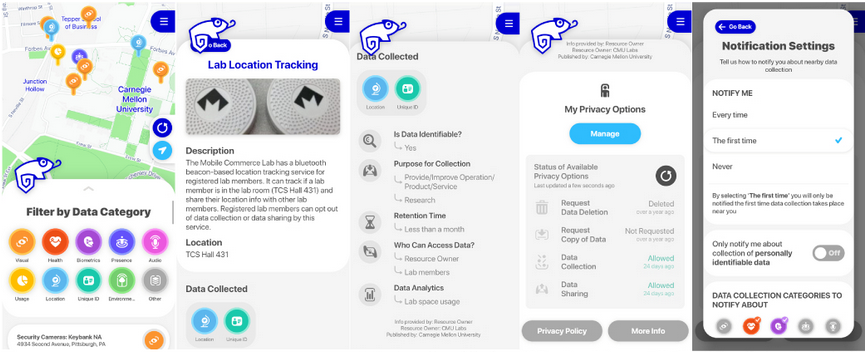
\includegraphics[width=734.25pt,height=298.5pt]{assets/images/iot_assistant.png}}
\end{picture}
\newpage
\begin{tikzpicture}[overlay]
\path(0pt,0pt);
\filldraw[color_283006][even odd rule]
(-15pt, 10pt) -- (945pt, 10pt)
-- (945pt, 10pt)
-- (945pt, -530pt)
-- (945pt, -530pt)
-- (-15pt, -530pt) -- cycle
;
\filldraw[color_214192][even odd rule]
(-15pt, -494pt) -- (945pt, -494pt)
-- (945pt, -494pt)
-- (945pt, -530pt)
-- (945pt, -530pt)
-- (-15pt, -530pt) -- cycle
;
\filldraw[color_252978][even odd rule]
(-15pt, -488.75pt) -- (945pt, -488.75pt)
-- (945pt, -488.75pt)
-- (945pt, -494pt)
-- (945pt, -494pt)
-- (-15pt, -494pt) -- cycle
;
\draw[color_155902,line width=0.5pt]
(79pt, -126.8751pt) -- (863.75pt, -126.8751pt)
;
\end{tikzpicture}
\begin{picture}(-5,0)(2.5,0)
\put(78.60001,-112.2741){\fontsize{48}{1}\selectfont\color{color_93343}Trabalho futuro}
\put(71.37503,-245.856){\fontsize{14}{1}\selectfont\color{color_252978}\unichar{9642}}
\put(86.82503,-245.856){\fontsize{20}{1}\selectfont\color{color_93343}Trabalhar na aplicação proposta.}
\put(71.37503,-281.456){\fontsize{14}{1}\selectfont\color{color_252978}\unichar{9642}}
\put(81.62503,-281.456){\fontsize{20}{1}\selectfont\color{color_93343}Possivelmente fazer uma recolha do conhecimento da população regional em relação à}
\put(78.57503,-303.1779){\fontsize{20}{1}\selectfont\color{color_93343}privacidade no mundo digital.}
\end{picture}
\newpage
\begin{tikzpicture}[overlay]
\path(0pt,0pt);
\filldraw[color_283006][even odd rule]
(-15pt, 10pt) -- (945pt, 10pt)
-- (945pt, 10pt)
-- (945pt, -530pt)
-- (945pt, -530pt)
-- (-15pt, -530pt) -- cycle
;
\filldraw[color_214192][even odd rule]
(-15pt, -494pt) -- (945pt, -494pt)
-- (945pt, -494pt)
-- (945pt, -530pt)
-- (945pt, -530pt)
-- (-15pt, -530pt) -- cycle
;
\filldraw[color_252978][even odd rule]
(-15pt, -488.75pt) -- (945pt, -488.75pt)
-- (945pt, -488.75pt)
-- (945pt, -494pt)
-- (945pt, -494pt)
-- (-15pt, -494pt) -- cycle
;
\draw[color_155902,line width=0.5pt]
(79pt, -126.8751pt) -- (863.75pt, -126.8751pt)
;
\end{tikzpicture}
\begin{picture}(-5,0)(2.5,0)
\put(78.60001,-112.2741){\fontsize{48}{1}\selectfont\color{color_93343}Obrigado}
\put(78.62503,-156.4779){\fontsize{20}{1}\selectfont\color{color_93343}Alguma questão?}
\end{picture}
\end{document}
